\documentclass[11pt,a4paper]{article}
\usepackage[T1]{fontenc}
\usepackage[utf8]{inputenc}
\usepackage[margin=24mm]{geometry}
\usepackage{lmodern,microtype,booktabs,graphicx,amsmath}
\usepackage{caption,hyperref}
\hypersetup{colorlinks=true,urlcolor=blue,citecolor=blue,linkcolor=blue,
pdftitle={Auditing a Small FER2013 Teaching Dataset},pdfauthor={Research manuscript draft}}
\setlength{\parskip}{4pt}
\setlength{\parindent}{0pt}
\setlength{\emergencystretch}{2em}
\title{Auditing a Small FER2013 Teaching Dataset:\\Source Recovery, Grouped Evaluation, and\\Controlled HOG--Transfer Learning Comparisons}
\author{Educational reproducibility study\\\small Author and affiliation to be confirmed before submission}
\date{12 November 2026 --- unsubmitted manuscript draft}
\begin{document}
\maketitle
\begin{abstract}
Small educational machine-learning projects can produce convincing accuracy
tables without establishing what their data or evaluation splits represent.
We reconstruct a 3,000-image facial-expression dataset and match every image
byte-for-byte to a versioned public FER2013 distribution. The reconstruction
identifies exact duplicates, conflicting annotations, reviewed near-duplicates,
and mixing of the distributor's training and test partitions. We produce locally
reviewable manifests, exclusion decisions, fixed grouped folds, and per-image
predictions, rather than treating historical scores on different splits as a
benchmark. A source-aligned retrospective extension compares HOG and a single
frozen ImageNet-pretrained ResNet18 representation under common linear and RBF
SVM heads, with nested grouped parameter selection and a training-majority
baseline. On a 509-image retrospective source-test subset, HOG--RBF and
ResNet18--RBF both achieve 39.49\% accuracy, with macro-F1 of 31.57\% and
35.28\%; the conditional paired interval for their macro-F1 difference includes
zero. Accuracy, macro-F1, per-class recall, confusion matrices, and paired
conditional bootstrap intervals expose both class imbalance and the limits of
small-sample comparisons. The contribution is an auditable educational case
study, not an architecture improvement, a new FER2013 leaderboard result, or
evidence of person-independent emotion inference.
\end{abstract}
\textbf{Keywords:} reproducibility; facial-expression classification; dataset
provenance; duplicate leakage; HOG; frozen transfer learning; grouped evaluation.

\section{Motivation and research questions}
A useful teaching study should explain how its conclusions depend on its data,
selection decisions, and measurement procedure. The recovered project originally
compared classical and CNN pipelines under different partitions. Those scores
cannot isolate a model effect. Adding a web interface would not repair this
problem; the present study instead reconstructs the experimental evidence.

We ask three bounded questions. \textbf{RQ1:} What can be verified about the
source, annotations, and independence of the recovered images?
\textbf{RQ2:} How do HOG and frozen CNN features compare when the classifier
family, parameter-selection budget, and evaluation examples are controlled?
\textbf{RQ3:} How much do aggregate accuracy, macro-F1, class-wise behavior,
and conditional uncertainty change the interpretation of the comparison?

The original contribution is the reconstruction and audit trail for this
particular teaching dataset, together with a reproducible controlled study.
HOG, ResNet, SVMs, nested validation, and the bootstrap are established methods.
No new descriptor, architecture, or general statistical procedure is proposed.
No classroom intervention or student-learning outcome was measured: educational
usefulness is a design motivation, not a demonstrated pedagogical effect.

\section{Context and related work}
FER2013 was introduced in the representation-learning challenges reported by
Goodfellow et al.~\cite{fer}. Their report is the bibliographic source for the
dataset family; it is not proof of the supply chain or photographic rights of
the recovered archive. We establish correspondence through file hashes.

Dalal and Triggs~\cite{hog} introduced HOG for human detection; here its use for
facial-expression labels is an application of a standard descriptor. Residual
networks~\cite{resnet} provide the learned representation. Work on ImageNet
transfer~\cite{transfer} motivates specifying the exact pretraining and transfer
configuration instead of treating ``CNN'' as a single method.

Near-duplicate auditing is established practice: Barz and Denzler~\cite{duplicates}
examined duplicate contamination in CIFAR. Their measured effects must not be
transferred numerically to this dataset. Our audit detects overlap but does not
estimate a causal amount of score inflation. Cross-validation fold errors are
dependent because training sets overlap; Bengio and Grandvalet~\cite{cvvariance}
explain why naive variance estimates can mislead. We therefore do not apply an
independent-fold $t$-test. Finally, image-category prediction is distinct from
inferring a person's internal emotional state, a distinction emphasized by
Barrett et al.~\cite{emotion}. The target here is the supplied image label.

\section{Data recovery and provenance}
\subsection{Recovered academic material}
The academic archive contains 2,000 historical training images, 700 historical
validation images, and 300 prediction images, all 48$\times$48 grayscale JPEGs.
The first 2,700 have labels; the remaining 300 lack academic ground truth.
All extracted JPEGs match the academic ZIP byte-for-byte. Two classical
checkpoints and historical reports were recovered; no historical CNN checkpoint
was recovered. In a separate reproducibility check, the historical HOG model
reproduces its 700-image validation accuracy (43.29\%) and macro-F1 (39.02\%).
This is a checkpoint-recovery result, not a clean comparison with a new CNN.

The 2,700 labels comprise angry 355, disgust 39, fear 413, happy 640, neutral
489, sad 451, and surprise 313. No person, capture-session, or demographic
metadata were found. Image grouping cannot establish person independence.

\subsection{Content-based source identification and licensing}
All 3,000 local files have an identical SHA-256 match in the public
\texttt{msambare/fer2013} Kaggle distribution, version 1~\cite{kaggle}.
The reference ZIP contains 35,887 images and has SHA-256
\texttt{9f3422c7a45b676c2965ef4fc5f3099932aa98fd13eaaa2c254f620a9894a6e9}.
This establishes content lineage to that distribution, not that the academic
packager obtained it from this uploader. The actual academic supply chain and
subset-sampling procedure remain undocumented.

Uploader metadata declares ``Database: Open Database, Contents: Database
Contents,'' mapped by Kaggle to ODbL 1.0 and Database Contents License
1.0~\cite{kagglelicenses,odbl,dbcl}. We record this declaration without claiming
independent verification of rights in each original photograph. This manuscript
reproduces no facial photographs. Code licensing and dataset licensing remain
separate. Reference labels are not used to fill the academic prediction set.

Content membership also shows that 2,324 local images match only distributor
\texttt{train}, 562 only \texttt{test}, and 114 both. Thus the local academic
split does not preserve the distributor split. Reference \texttt{test} is not
treated here as one untouched external cohort, nor is it a different domain.
Among labeled files, 2,691 have unanimous reference-label agreement and nine
have exact reference copies with different labels, at least one agreeing with
the academic label. No automatic relabeling was performed.

\subsection{Duplicates, review, and exclusion decisions}
Exact matching identifies 20 groups covering 42 images (22 excess copies), with
seven groups crossing the historical training--validation split. Three groups
link labeled images to the 300-image prediction set. Exact and decoded-pixel
hashes are recorded in the manifests.

An additional 64-bit horizontal difference-hash screen (Hamming distance at most
four) produces 126 non-exact candidate pairs. A single assistant visual review,
supported by similarity diagnostics, labels 37 as photographic near-duplicates,
87 as different images, and two as uncertain. These are image-reuse judgments,
not facial identity judgments. Screening may miss transformed copies; the review
has no second independent human rater or inter-rater agreement estimate.

Connected components combine exact pairs, reviewed near-duplicates, and uncertain
pairs conservatively. They form 39 multi-image groups containing 91 IDs. The
selection ledger excludes 13 labeled images in conflicting-label components,
three labeled images in uncertain components, and seven additional labeled
images linked to the prediction set. The resulting 2,677-image eligible inventory
retains same-label copies within groups. Metrics therefore weight images, not
unique photographs. Exclusions are documented decisions, not ground-truth
corrections or proof that all remaining data are clean.

\section{Evaluation design}
\subsection{Evidence stages and the source-aligned cohort}
We preserve three distinct stages. Historical reports use their original,
incomparable partitions. The first reconstructed experiment (v1) uses one common
1,605/536/536 grouped train/validation/test split of the 2,677-image inventory.
It is retrospective because the labeled pool was previously explored. A later
source investigation motivates the present v2 extension. V1 outputs are not
overwritten or presented as original FER2013 benchmark scores.

V2 restricts development to 2,069 eligible images whose exact reference matches
occur only in distributor \texttt{train}. The 96 eligible images matching both
reference partitions are excluded. Of 512 eligible source-test-only images,
three have reviewed image groups present in development and are excluded from
evaluation. The remaining 509 form the source-test subset. No new reference
images are added and no academic prediction labels are recovered from reference
classes. All local labeled examples were accessible in earlier work; the 509
images are held out of v2 model fitting, but are \emph{not historically untouched}.

\begin{table}[ht]
\centering
\caption{V2 cohort construction from the 2,677-image eligible inventory.}
\begin{tabular}{lr}\toprule
Role & Images \\\midrule
Development: source-train-only & 2069 \\
Excluded: exact content in both source partitions & 96 \\
Excluded: known group crosses development/source-test & 3 \\
Retrospective source-test subset & 509 \\\bottomrule
\end{tabular}
\end{table}

\subsection{Common representations and classifier controls}
HOG uses grayscale floats divided by 255, nine orientations, 8$\times$8 cells,
2$\times$2-cell blocks, and L2-Hys normalization on 48$\times$48 inputs, producing
900 features. ResNet18 uses the official torchvision ImageNet1K V1 weights
(SHA-256 recorded in the protocol), fixed in evaluation mode, with its final
classifier replaced by identity. Official transforms resize the shorter side
to 256, center-crop 224, convert to RGB tensor, and apply ImageNet normalization.
Upsampling introduces no new facial detail. Global pooled features have 512
dimensions. There is no fine-tuning or augmentation.

Both representations use a linear-kernel SVC and an RBF SVC, each preceded by
StandardScaler fitted only on the current training fold. RBF uses
\texttt{gamma=scale}; both heads search $C\in\{0.1,1,10\}$, with no class
weighting. The control fixes classifier families and search budgets, but does
not equalize feature dimensionality, extraction cost, information available
through ImageNet pretraining, or effective kernel geometry. In particular,
\texttt{gamma=scale} adapts to feature scale and dimensionality.

The baseline predicts the training-fold majority label, breaking ties
lexicographically. The v1 CNN instead trained a linear neural head; it is not
silently equated with the v2 SVM head. LBP and additional CNN architectures are
outside the new controlled comparison.

\subsection{Nested grouped selection and exported measurements}
Five shared outer StratifiedGroupKFold partitions produce one out-of-fold (OOF)
prediction per development image. Each outer training pool uses three shared
inner grouped folds. Mean inner macro-F1 selects $C$; an exact tie selects the
smaller value. The scaler is re-fitted within every inner training fold. For the
source-test subset, a separate three-fold grouped search on all development
images selects $C$, then fits once on all development images. The same evaluation
IDs and labels are used for every pipeline within each evaluation scope.

Seeds and all inner/outer ID lists were frozen in a dated v2 analysis plan before
v2 outcome computation. This is a local analysis plan, not public preregistration;
its design was informed by the earlier v1 results. Fixed, unsupervised feature
extraction is cached once; no target-fitted representation or scaler is cached
across folds. The four pipelines require 240 SVM fits including final fits.

Primary reporting uses pooled per-image OOF macro-F1, with accuracy, class recall,
supports, and confusion matrices. Macro-F1 is the unweighted mean of seven
class-specific F1 scores, using zero for a zero denominator. Pooled OOF macro-F1
need not equal mean fold macro-F1 because F1 is nonlinear. Fold scores are
exported descriptively, without treating folds as independent replications.

\subsection{Conditional uncertainty and interpretation}
We resample known image groups with replacement within each true-label stratum
for 2,000 paired bootstrap replicates, preserving all images in a sampled group.
The estimand remains per-image performance. All pipelines use identical sampled
groups. We report percentile 95\% intervals and, for four prespecified paired
contrasts, 98.75\% intervals as a Bonferroni multiplicity convention per metric
within each scope. These nominal intervals are approximate, not exact tests.

Resampling saved predictions conditions on realized training, parameter
selection, and folds. It does not propagate training-set, split-selection,
hyperparameter-selection, pretraining, or reviewer uncertainty. In OOF analysis
it also does not account for dependence from overlapping training folds.
Unknown same-person dependencies remain. We use intervals as descriptive
uncertainty summaries and avoid claims of population-level algorithm superiority.

\section{Results}
\subsection{Common-split v1 results retained as context}
On the v1 536-image internal test, the majority baseline achieves 23.88\%
accuracy and 5.51\% macro-F1. HOG--RBF reaches 38.62\% and 35.79\%, while the
frozen ResNet18 with trained neural linear head reaches 40.49\% and 31.71\%.
Higher accuracy therefore does not imply higher macro-F1. These are single-split,
single-seed results; they do not estimate initialization variability or justify
a universal classical-versus-CNN ranking.

\subsection{Source-aligned classifier controls}
Table~\ref{tab:scores} reports the new v2 results with a common evaluation set
for every pipeline. Figure~\ref{fig:f1} visualizes their conditional intervals.
Paired differences are exported separately, so overlap of marginal intervals
is not used as a test of a model difference. The source-test and OOF scopes have
different images and training-pool sizes; their difference is not an estimated
causal effect of the partitioning rule.

\begin{table}[ht]
\centering\small
\caption{V2 accuracy and macro-F1 in percent. Intervals resample known image
groups conditional on predictions; see the uncertainty limitations.}
\label{tab:scores}
\begin{tabular}{llrr}
\toprule
Evaluation & Pipeline & Accuracy & Macro-F1 [95\% interval] \\
\midrule
OOF & Majority & 24.55 & 5.63 [5.61, 5.66] \\
OOF & HOG + linear SVM & 28.66 & 25.20 [22.76, 27.64] \\
OOF & HOG + RBF SVM & 39.29 & 30.96 [29.12, 32.82] \\
OOF & ResNet18 + linear SVM & 37.60 & 32.63 [30.36, 34.90] \\
OOF & ResNet18 + RBF SVM & 44.03 & 36.92 [34.50, 39.63] \\
Source-test & Majority & 24.75 & 5.67 [5.67, 5.67] \\
Source-test & HOG + linear SVM & 30.84 & 27.58 [23.08, 32.78] \\
Source-test & HOG + RBF SVM & 39.49 & 31.57 [28.00, 35.17] \\
Source-test & ResNet18 + linear SVM & 33.99 & 30.11 [25.45, 35.03] \\
Source-test & ResNet18 + RBF SVM & 39.49 & 35.28 [29.65, 41.10] \\
\bottomrule
\end{tabular}

\end{table}

\begin{figure}[ht]
\centering
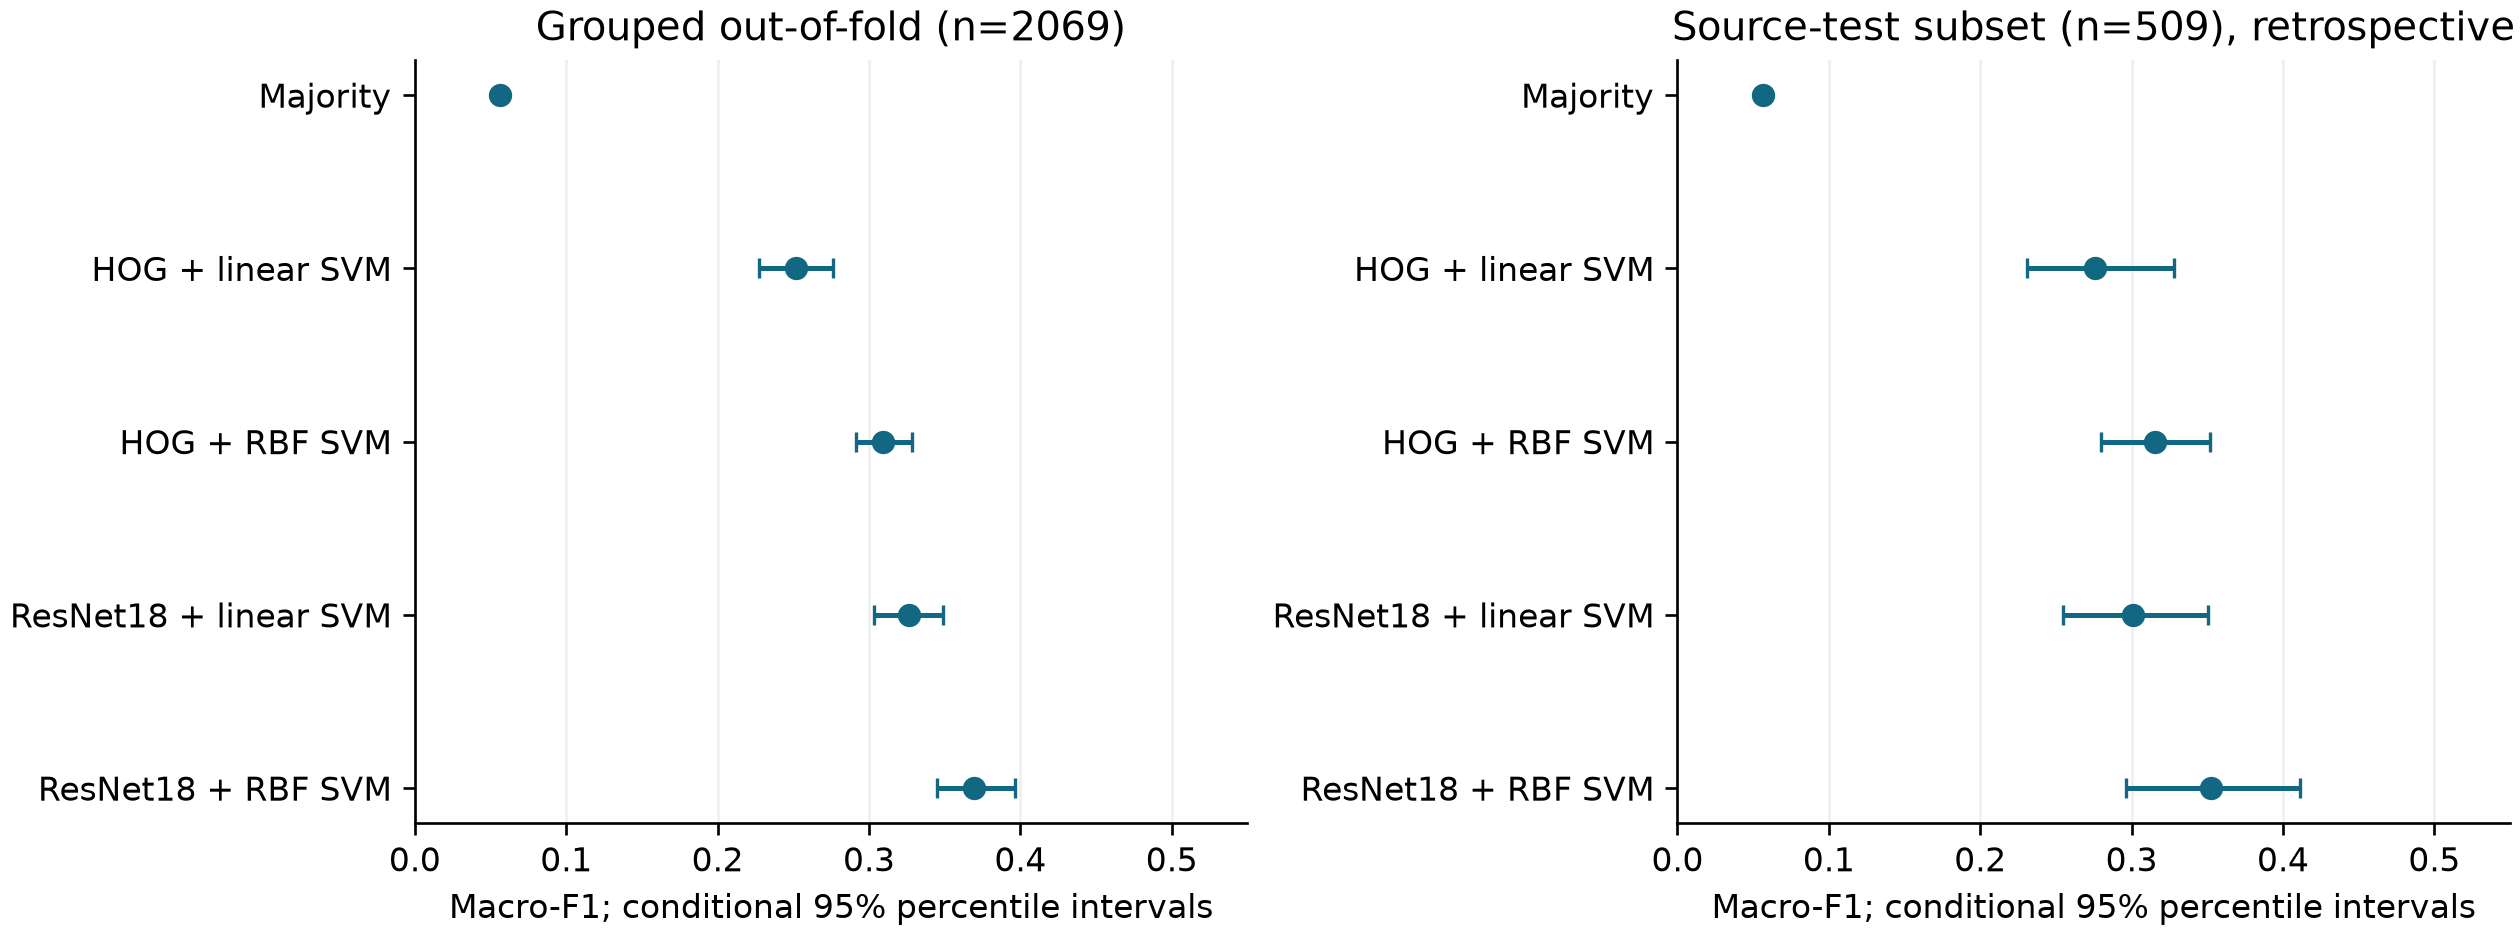
\includegraphics[width=\linewidth]{../studiu_v2/results/macro_f1.png}
\caption{Macro-F1 and conditional 95\% intervals. A frozen CNN representation
is evaluated with common SVM heads. The source-test subset is retrospective.}
\label{fig:f1}
\end{figure}

For pooled OOF predictions, ResNet18--RBF reaches 44.03\% accuracy and 36.92\%
macro-F1, compared with 39.29\% and 30.96\% for HOG--RBF. Their macro-F1
difference is 5.96 percentage points, with a conditional paired 95\% interval
of [3.17, 8.76] points and a four-comparison interval of [2.57, 9.59].
These intervals describe the saved predictions; they do not establish a
population-level advantage after accounting for training-fold dependence.

On the separate 509-image source-test subset, both RBF pipelines correctly
classify 201 images (39.49\% accuracy). Their macro-F1 values nevertheless
differ: 31.57\% for HOG and 35.28\% for ResNet18. The paired macro-F1 difference
is 3.71 points, with a 95\% interval of [-2.35, 9.72] and a four-comparison
interval of [-4.19, 11.89]. This sample does not resolve a clear advantage in
that comparison under the stated resampling scheme. Equal total correct counts
do not imply identical errors or class-wise performance.

Changing the head also matters. OOF macro-F1 increases from 25.20\% to 30.96\%
for HOG when using RBF instead of linear, and from 32.63\% to 36.92\% for
ResNet18. Thus a comparison with unmatched heads would conflate representation
and classifier effects. Final development-only selection chooses $C=0.1$ for
both linear heads and $C=10$ for both RBF heads. These selections are exported
with every inner-fold score, including unsuccessful candidates.

The majority baseline yields 24.75\% accuracy but only 5.67\% macro-F1 on the
source-test subset. Its degenerate conditional interval is a consequence of
class-stratified resampling with fixed class counts in this cohort, not proof
that its population performance has no uncertainty. All four learned pipelines
exceed this simple baseline in point estimates, while none approaches a reliable
seven-class deployment system.

The complete v2 run, including fixed extraction, selection, prediction, and
bootstrap summaries, took 114.80 seconds on this machine. Recorded feature
extraction took 0.95 seconds for HOG and 27.18 seconds for the frozen ResNet18
over all 2,578 active images. These one-run cached batch timings are descriptive
and are not a replicated speed benchmark.


\subsection{Class-wise errors}
\begin{table}[ht]
\centering\small
\caption{Recall in percent on the 509-image retrospective source-test subset.
Support is shown explicitly; disgust contains only eight examples.}
\label{tab:recall}
\begin{tabular}{lrrrrr}
\toprule
Class (support) & Majority & HOG lin. & HOG RBF & RN lin. & RN RBF \\
\midrule
angry (81) & 0.0 & 22.2 & 18.5 & 28.4 & 17.3 \\
disgust (8) & 0.0 & 12.5 & 0.0 & 12.5 & 12.5 \\
fear (77) & 0.0 & 33.8 & 27.3 & 33.8 & 29.9 \\
happy (126) & 100.0 & 42.9 & 67.5 & 47.6 & 57.9 \\
neutral (87) & 0.0 & 32.2 & 46.0 & 35.6 & 41.4 \\
sad (80) & 0.0 & 21.2 & 27.5 & 21.2 & 41.2 \\
surprise (50) & 0.0 & 26.0 & 36.0 & 30.0 & 42.0 \\
\bottomrule
\end{tabular}

\end{table}

Class-wise recall and full confusion counts prevent a strong majority-class
result from concealing failure on rare labels. Each disgust error changes recall
by 12.5 percentage points in this source-test subset. Zero recall is a measured
failure for that class in this sample, not evidence that its population recall
is exactly zero. Error patterns cannot establish annotation correctness or an
underlying psychological mechanism.

\begin{figure}[p]
\centering
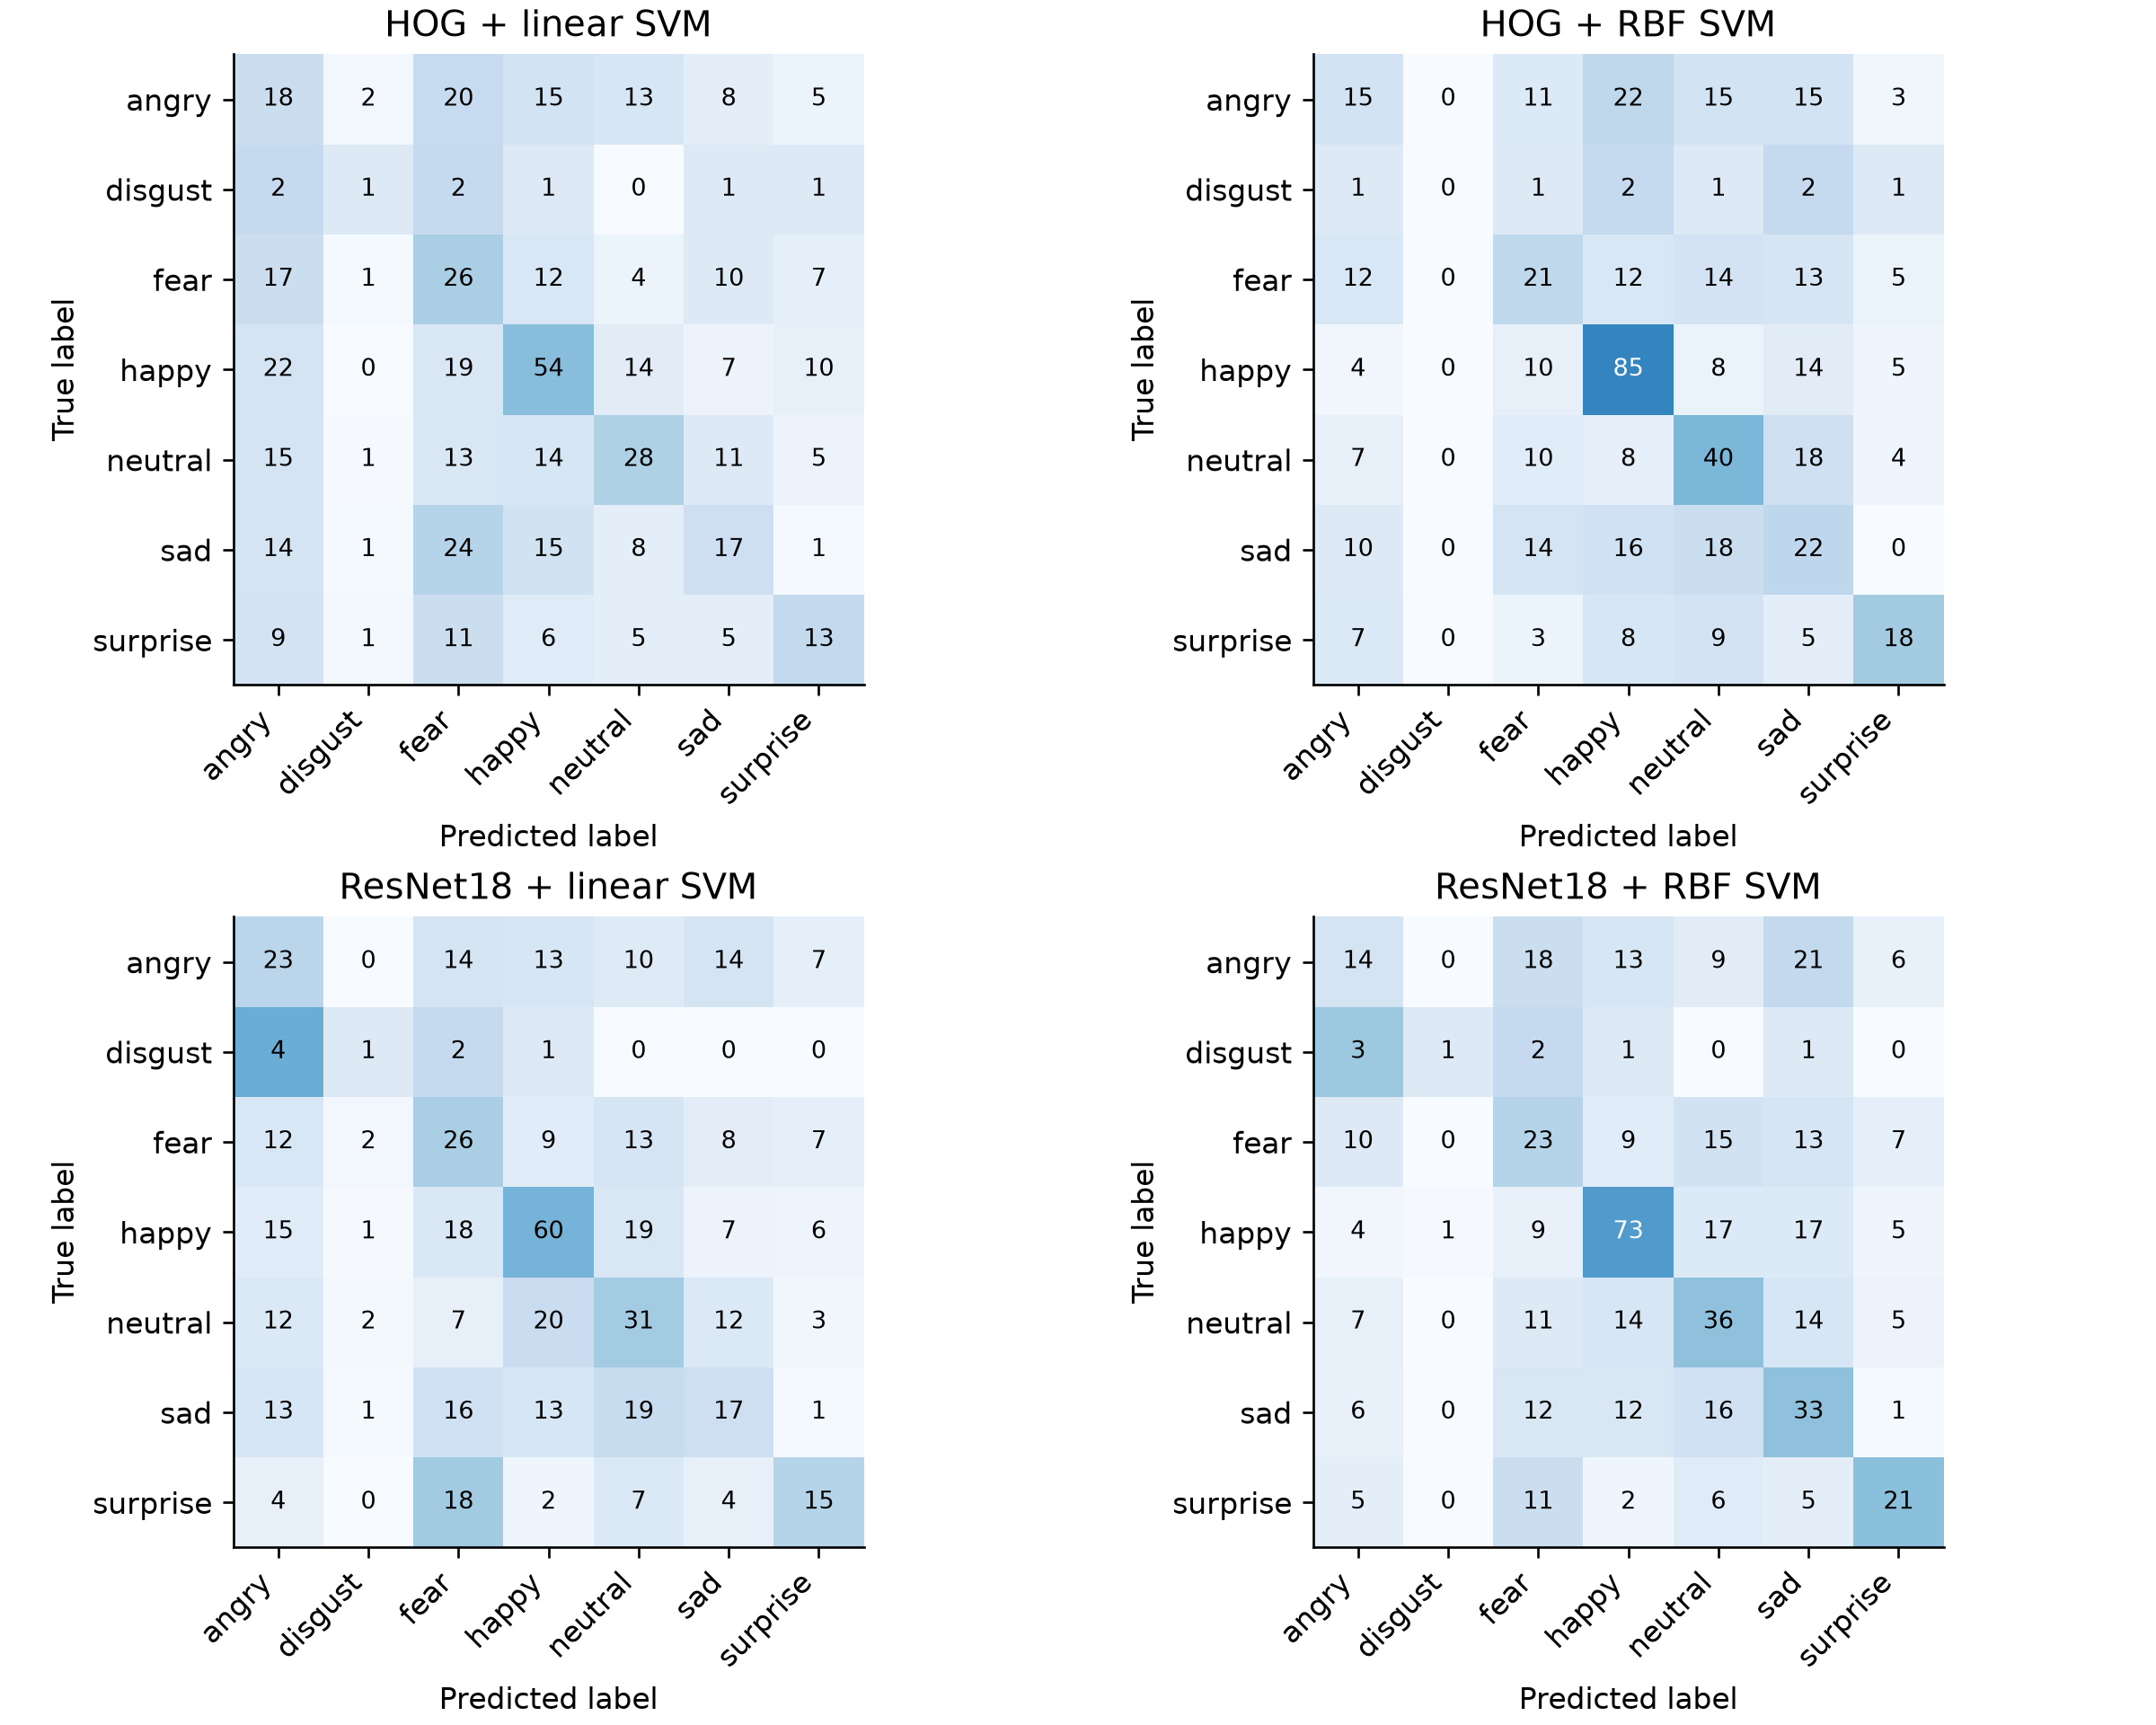
\includegraphics[width=.96\linewidth]{../studiu_v2/results/confusion_holdout.png}
\caption{Source-test subset confusion matrices. Rows are true labels and columns
predictions. Printed values are counts; background intensity is row-normalized
on a common zero-to-one scale. No individual facial photographs are reproduced.}
\label{fig:confusion}
\end{figure}

\section{Reproducibility and practical cost}
The evidence package includes ID/label/hash/group manifests, source correspondence,
an exclusion ledger, all folds, a frozen configuration and code hashes,
hyperparameter-selection traces, and raw OOF/source-test predictions. A verifier
rechecks image hashes and artifact integrity and recomputes metrics and bootstrap
summaries without network access or model fitting. Synthetic tests check grouping,
metric formulas, and paired-bootstrap behavior. Integrity hashes detect changes;
they do not prove that the underlying design or annotations are correct.

Before v2 fitting, a cost-only pilot used 140 development images and reported
approximately 65 seconds for all CNN feature extraction by linear extrapolation.
The planned CPU budget was 5--15 minutes for extraction and 240 SVM fits, with a
15-minute stop policy at fold boundaries. All extraction is CPU-based with at
most four Torch threads on an Intel Core i5-13600KF. Feature caching avoids
repeating the frozen backbone for each hyperparameter candidate. Exact versions,
observed elapsed time, and separate extraction timings are in the results JSON.
These batch measurements are not interactive request latency, throughput under
load, or an end-to-end real-time measurement.

Reproduction requires recovering the academic archive and verified local
pretrained weights; neither is embedded in the manuscript. The source matching
procedure additionally requires the versioned public reference ZIP and saved
metadata. The run instructions distinguish numerical verification of saved
predictions from full model retraining. No claim of cross-platform bitwise
identity is made.

\section{Threats to validity and responsible scope}
\textbf{Sampling and external validity.} The 3,000-image academic sampling
procedure is unknown. A small subset of FER2013 cannot support conclusions for
all FER2013, video, deployment cameras, demographic groups, or other datasets.
There is no independent cross-dataset evaluation and no subject-disjoint claim.
Potential overlap between ImageNet pretraining and facial images was not audited.

\textbf{Retrospective analysis.} Earlier project work and v1 fitting accessed
the labeled pool. The v2 plan controls the new fitting workflow but cannot
restore historical blindness. Selecting a small $C$ grid, representations, and
review rules constitutes researcher choice, not a globally optimized comparison.
No additional configurations were chosen after viewing the v2 results.

\textbf{Duplicates and annotations.} Hashes find exact copies; the difference-hash
screen and one assistant review are incomplete. Grouping by image does not group
all images of a person. Excluding conflicts changes the target population and
does not establish that retained labels are correct. Bootstrap strata condition
on observed class/group counts and do not quantify prevalence uncertainty.

\textbf{Statistical reach.} One fixed five-fold partition does not establish
split robustness. Deterministic SVM fits do not measure stochastic CNN
fine-tuning variability. Conditional intervals exclude important sources of
uncertainty and cannot certify an algorithm ranking. No duplicate-removal
performance difference is interpreted causally.

\textbf{Construct and ethics.} The seven targets are dataset annotation categories,
not verified internal emotional states. We recruited no participants, collected
no new faces, inferred no identities, and measured no psychological or medical
outcome. Consent history, original photo rights, demographic fairness, and
appropriate deployment are not established by this audit. The work does not
justify surveillance, student assessment, medical use, or automated judgments
about people.

\section{Contribution and remaining publication work}
The study supplies a concrete example of repairing a teaching comparison through
provenance recovery, explicit exclusions, grouped selection, classifier controls,
and inspectable predictions. Its central lesson is methodological: a reproducible
finding includes the conditions and limitations under which it was obtained.
The new experiment should be read as evidence for this subset and these fixed
configurations, without architecture novelty or benchmark-superiority claims.

Before submission, the author must confirm authorship and affiliation, obtain a
second independent review of duplicate decisions, check the intended venue's
requirements, and resolve what data or derivatives may be distributed. Academic
official test labels remain missing; these are needed only for a separately
authorized official-test evaluation. Stronger external claims would require a
new independently sourced, appropriately licensed, subject-aware dataset and a
fresh evaluation plan. Those results are not implied by the present manuscript.

\paragraph{Data and code availability.} This is a local, unsubmitted draft.
No data archive, checkpoint, manuscript, or code release has been published by
this work. The accompanying local repository contains the analysis code and
numeric evidence; availability statements must be updated only after an actual
authorized release. The manuscript contains no unverifiable public archive DOI.

\paragraph{AI assistance and author verification.} An AI coding assistant helped
recover and audit artifacts, implement the evaluation, inspect duplicate
candidates, and draft the manuscript. The single assistant review is explicitly
distinguished from independent human annotation. A human author must verify the
claims, references, authorship, and applicable venue disclosure policy before
submission. No author approval, ethics approval, or funding statement is asserted.

\begingroup
\small
\setlength{\parskip}{0pt}
\begin{thebibliography}{12}
\setlength{\itemsep}{3pt}
\bibitem{fer} I. J. Goodfellow et al. Challenges in Representation Learning:
A report on three machine learning contests. 2013.
\url{https://arxiv.org/abs/1307.0414}.
\bibitem{hog} N. Dalal and B. Triggs. Histograms of Oriented Gradients for Human
Detection. CVPR, pp. 886--893, 2005.
\url{https://lear.inrialpes.fr/people/triggs/pubs/Dalal-cvpr05.pdf}.
\bibitem{resnet} K. He, X. Zhang, S. Ren, and J. Sun. Deep Residual Learning for
Image Recognition. CVPR, pp. 770--778, 2016.
\url{https://arxiv.org/abs/1512.03385}.
\bibitem{transfer} S. Kornblith, J. Shlens, and Q. V. Le. Do Better ImageNet
Models Transfer Better? CVPR, 2019. \url{https://arxiv.org/abs/1805.08974}.
\bibitem{duplicates} B. Barz and J. Denzler. Do We Train on Test Data? Purging
CIFAR of Near-Duplicates. Journal of Imaging 6(6):41, 2020.
\url{https://doi.org/10.3390/jimaging6060041}.
\bibitem{cvvariance} Y. Bengio and Y. Grandvalet. No Unbiased Estimator of the
Variance of K-Fold Cross-Validation. JMLR 5:1089--1105, 2004.
\url{https://jmlr.org/papers/v5/grandvalet04a.html}.
\bibitem{emotion} L. F. Barrett, R. Adolphs, S. Marsella, A. M. Martinez, and
S. D. Pollak. Emotional Expressions Reconsidered: Challenges to Inferring Emotion
From Human Facial Movements. Psychological Science in the Public Interest
20(1), 2019. \url{https://doi.org/10.1177/1529100619832930}.
\bibitem{kaggle} M. Sambare. FER-2013, Kaggle distribution, version 1, 2020.
Saved metadata and content verified locally in November 2026.
\url{https://www.kaggle.com/datasets/msambare/fer2013}.
\bibitem{kagglelicenses} Kaggle. Dataset Metadata: license identifiers.
\url{https://github.com/Kaggle/kaggle-api/blob/main/docs/datasets_metadata.md}.
\bibitem{odbl} Open Data Commons. Open Database License 1.0.
\url{https://opendatacommons.org/licenses/odbl/1-0/}.
\bibitem{dbcl} Open Data Commons. Database Contents License 1.0.
\url{https://opendatacommons.org/licenses/dbcl/1-0/}.
\end{thebibliography}
\endgroup
\end{document}
